\chapter{Implementasi dan Pengujian}

Pada bab ini, akan dibahas implementasi dari modifikasi pengoptimasi yang sebelumnya telah dibahas, serta perbandingannya dengan penelitian dari \textcite{Chen2022Efficient} dan \textcite{Chen2021CADA}.

\section{Implementasi}
Algoritma pengoptimasi yang dijelaskan dalam penelitian \textcite{Chen2022Efficient} dan \textcite{Chen2021CADA} masing-masing akan diimplementasikan menggunakan pustaka PyTorch dengan arsitektur \emph{parameter server}. Kemudian, implementasi modifikasi penggabungan akan didasarkan kepada hasil implementasi kedua pengoptimasi.

Setiap pengoptimasi akan dibagi menjadi tiga bagian, yakni \emph{parameter server}, \emph{trainer}, dan \emph{runner}. Bagian \emph{parameter server} memiliki tugas umum menjadi \emph{node} yang menyimpan model utama. Kemudian, \emph{trainer} akan mendapatkan parameter model dari \emph{parameter server} dan melakukan perhitungan gradien. Gradien yang telah dihitung lalu dikirim kembali kepada \emph{parameter server} untuk memperbarui parameter model. Bagian yang akan mengorkestrasi hubungan ini adalah \emph{runner}.

Algoritma untuk pengoptimasi gabungan akan dibagi menjadi 2, yakni bagian \textit{parameter server} serta bagian \textit{worker}. Algoritma untuk \textit{parameter server} dapat dilihat pada algoritma~\ref{myadam_server}. Algoritma untuk \textit{worker} dapat dilihat pada algoritma~\ref{myadam_worker}. Kondisi yang digunakan untuk menentukan pengiriman dari tiap \textit{worker} dapat dilihat pada persamaan~\ref{cada2cond}.

\begin{equation}
  \label{cada2cond}
  \|\nabla f_t(\theta_t) - \nabla f_t(\theta_{t-\tau})\|^2 \leq \frac{c}{D} \sum_{d=1}^{D} \|\theta_{t+1-d} - \theta_{t-d}\|^2
\end{equation}

\begin{algorithm}[ht]
  \setstretch{1}
  \caption{Modifikasi Adam untuk Parameter Server}\label{myadam_server}
  \begin{algorithmic}[1]
    \State \textbf{Parameter:} Fungsi Kuantisasi $\mathcal{Q}_s$
    \State \textbf{Inisialisasi} vektor parameter $\theta_0$, error term $e_1 \gets 0$
    \State Sebarkan $\theta_0$ ke semua \textit{worker}
    \For{$t = 1,2,\dots,T$}
    \State $\hat{\delta_t} \gets \textnormal{rata-rata } \delta_t^{(i)}$ dari setiap \textit{worker}
    \State Sebarkan $\tilde{\delta_t} \gets \mathcal{Q}(\hat{\delta_t} + e_t)$
    \State $e_{t+1} \gets e_{t}$
    \State $\theta_{t+1} \gets \theta_t - \tilde{\delta_t}$
    \EndFor
  \end{algorithmic}
\end{algorithm}

\begin{algorithm}[ht]
  \caption{Modifikasi Adam untuk Worker ke-$i$}\label{myadam_worker}
  \setstretch{1}
  \begin{algorithmic}[1]
    \State \textbf{Parameter:} Fungsi Kuantisasi $\mathcal{Q}_w$, Hyperparameter Adam $\alpha, \beta_1, \beta_2$, konstanta batas $c$, batas maksimum penundaan $D$
    \State $m_0^{(i)} \gets 0, v_0^{(i)} \gets \epsilon, e_1^{(i)} \gets 0, \tau^{(i)} \gets 0$
    \State $\theta^{(i)}_0 \gets \theta_1$ dari server
    \For{$t=1,2,\dots,T$}
    \State $g_t^{(i)} \gets \nabla_\theta f_t(\theta_{t})$
    \State $v_t^{(i)} \gets \theta_t v_{t-1}^{(i)} + (1-\theta_t)[g_t^{(i)}]^2$
    \State $m_t^{(i)} \gets \beta_1 m_{t-1}^{(i)} + (1-\beta_1)g_t^{(i)}$
    \State $\alpha_t \gets \alpha \sqrt{1-\beta_2^t}/(1-\beta_1^t)$
    \State $\delta^{(i)} \gets \alpha_t m_t^{(i)}/\sqrt{v_t^{(i)}}+e_t^{(i)}$
    \State $\theta_t \gets \theta_{t-1} - \delta^{(i)}$
    \State Hitung $\nabla f_t(\theta^{(i)}_{t})$ dan $\nabla f_t(\theta^{(i)}_{t-\tau})$
    \State $\delta^{(i)} \gets \mathcal{Q}_w(\delta^{(i)})$
    \If{Kondisi \ref{cada2cond} tidak terpenuhi atau $\tau \ge D$}
    \State Kirim $\delta^{(i)}$
    \State $\tau \gets 1$
    \Else
    \State $\tau \gets \tau + 1$
    \EndIf
    \State $e_{t+1}^{(i)} \gets \alpha_t \frac{m_t^{(i)}}{\sqrt{v_t^{(i)}}} + e_t^{(i)} - \delta_t^{(i)}$
    \State Terima $\tilde{\delta_t}$ dari server
    \State $\theta_{t} \gets \theta_{t-1} - \tilde{\delta_t}$
    \EndFor
  \end{algorithmic}
\end{algorithm}

\section{Pengujian}
\subsection{Lingkungan Pengujian}
Pengujian dilakuan pada server DGX dengan spesifikasi pada tabel~\ref{dgx}. Namun, pengujian dilakukan dengan melakukan simulasi \emph{deep learning} terdistribusi pada hanya satu GPU.

\begin{table}[ht]
  \caption{Spesifikasi Lingkungan Pengujian}\label{dgx}
  \centering
  \setstretch{1.5}
  \begin{tabular}[ht]{ | c | c | }
    \hline
    \textbf{Parameter} & \textbf{Spesifikasi}                           \\
    \hline
    CPU                & 2x Intel Xeon E5-2698 v3 (16-core, Haswell-EP) \\
    \hline
    RAM                & 512GB DDR4-2133                                \\
    \hline
    GPU                & 8x Tesla V100 32GB VRAM                        \\
    \hline
    Penyimpanan        & 4x1.92 TB SSD                                  \\
    \hline
  \end{tabular}
\end{table}

Selain itu, versi perangkat lunak dan pustaka dapat dilihat pada tabel~\ref{softwares}.
\begin{table}[ht]
  \caption{Versi Perangkat Lunak}\label{softwares}
  \centering
  \setstretch{1.5}
  \begin{tabular}{ | c | c | }
    \hline
    \textbf{Perangkat Lunak} & \textbf{Versi} \\
    \hline
    Python                   & 3              \\
    \hline
    PyTorch                  & 1.13.1+cuda    \\
    \hline
    TorchVision              & 0.14.1+cuda    \\
    \hline
  \end{tabular}
\end{table}

\subsection{Skenario Pengujian}
Pengujian dilakukan dengan melatih model ResNet-20 pada \emph{dataset} CIFAR10. Model ResNet-20 diambil dari \emph{repository} GitHub \cite{Idelbayev18a} dengan beberapa perubahan agar dapat digunakan pada CPU dan GPU. Kemudian \emph{dataset} CIFAR10 didapatkan menggunakan pustaka Torchvision.

Pemilihan \emph{hyperparameter} untuk masing-masing teknik dapat dilihat pada tabel~\ref{hyperparam}. Selain itu, untuk teknik Efficient-Adam dari \textcite{Chen2022Efficient} serta teknik gabungan, fungsi kuantisasi yang digunakan adalah menggunakan pemetaan langsung ke tipe data \emph{float16} pada PyTorch.

\begin{table}[ht]
  \caption{Pemilihan \emph{Hyperparameter}}\label{hyperparam}
  \centering
  \setstretch{1.5}
  \begin{tabular}{ | c | c | c | }
    \hline
    \textbf{Teknik}                                               & \textbf{Parameter} & \textbf{Nilai} \\
    \hline
    \multirow{5}{*}{CADA, \textcite{Chen2021CADA}}                & $\alpha$           & 0.01           \\
                                                                  & $\beta_1$          & 0.9            \\
                                                                  & $\beta_2$          & 0.99           \\
                                                                  & $D$                & 50             \\
                                                                  & $d_{max}$          & 2              \\
                                                                  & $c$                & 0.12           \\
    \hline
    \multirow{3}{*}{Efficient-Adam, \textcite{Chen2022Efficient}} & $\alpha$           & 0.0005         \\
                                                                  & $\beta_1$          & 0.9            \\
                                                                  & $\beta_2$          & 0.999          \\
    \hline
    \multirow{5}{*}{Gabungan}                                     & $\alpha$           & 0.0005         \\
                                                                  & $\beta_1$          & 0.9            \\
                                                                  & $\beta_2$          & 0.999          \\
                                                                  & $D$                & 50             \\
                                                                  & $d_{max}$          & 2              \\
                                                                  & $c$                & 0.12           \\
    \hline
  \end{tabular}
\end{table}

Pengujian dilakukan dengan merekam jumlah byte yang dipertukarkan serta jumlah komunikasi yang dilakukan antara \emph{parameter server} dengan \emph{trainer}. Selain itu, akurasi dan nilai \emph{loss} setiap \emph{epoch} akan direkam untuk membandingkan hasil model. Pengujian dilakukan untuk masing-masing teknik secara terpisah menggunakan parameter yang ditentukan.

\subsection{Hasil Pengujian}

Hasil yang akan dibandingkan dalam pengujian utamanya adalah jumlah komunikasi serta jumlah byte yang digunakan untuk komunikasi. Namun, akurasi model juga akan dibandingkan untuk memastikan setiap teknik mampu menghasilkan model dengan kemampuan yang mirip. Plot akurasi tiap epoch untuk ketiga teknik dapat dilihat pada gambar~\ref{acc}. Dalam plot tersebut dapat dilihat akurasi model yang dihasilkan ketiga teknik berada di atas 80\%, dengan Efficient-Adam dari \textcite{Chen2022Efficient} terletak sedikit lebih di atas kedua teknik lainnya.

\begin{figure}[ht]
  \centering
  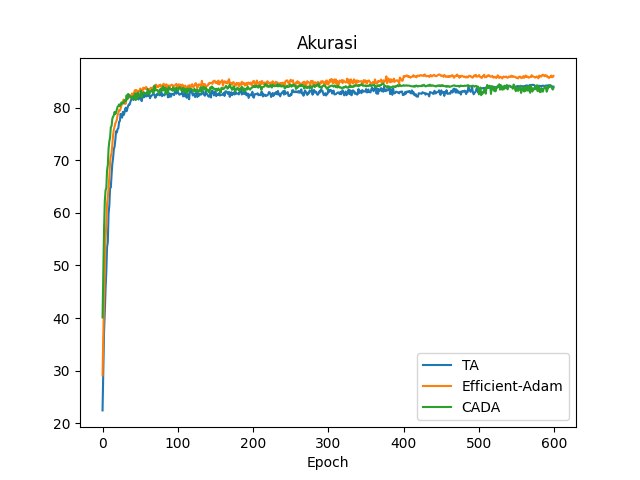
\includegraphics[width=0.8\textwidth]{acc.png}
  \caption{Akurasi tiap teknik}\label{acc}
\end{figure}

Plot perbandingan jumlah komunikasi untuk tiap teknik dapat dilihat pada gambar~\ref{comms}. Dalam plot tersebut, terlihat bahwa teknik Efficient-Adam sangat berimpitan dengan CADA. Namun, teknik CADA mampu mengurangi jumlah komunikasi dalam skala kecil, masih tetap di atas 975 komunikasi. Di sisi lain, implementasi gabungan memberikan pengurangan jumlah komunikasi yang cukup banyak, hingga hanya membutuhkan kurang dari 825 komunikasi di sebelum epoch 600.

\begin{figure}[ht]
  \centering
  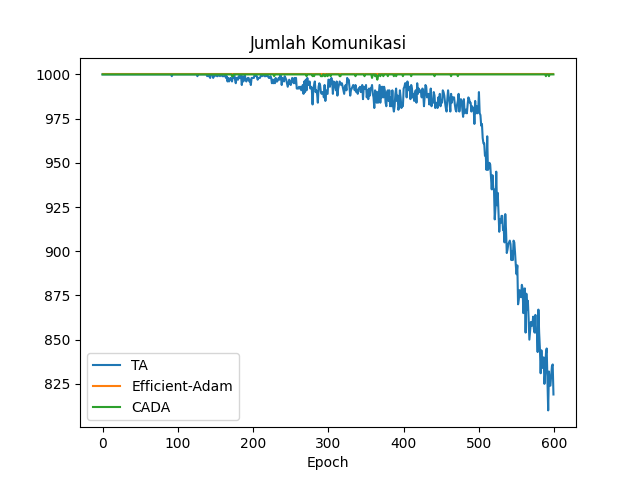
\includegraphics[width=0.8\textwidth]{comms.png}
  \caption{Jumlah komunikasi tiap teknik}\label{comms}
\end{figure}

Plot perbandingan jumlah byte yang digunakan dapat dilihat pada gambar~\ref{bits}. Dapat dilihat bahwa jumlah byte yang digunakan oleh CADA sekitar 4 kali lebih besar dibandingkan Efficient-Adam serta teknik gabungan. Namun, terlihat bahwa teknik gabungan menggunakan lebih banyak byte dibandingkan Efficient-Adam saja. Kemudian, jumlah byte yang digunakan oleh teknik gabungan terlihat berkurang sesuai dengan pengurangan jumlah komunikasi yang terjadi.

\begin{figure}[ht]
  \centering
  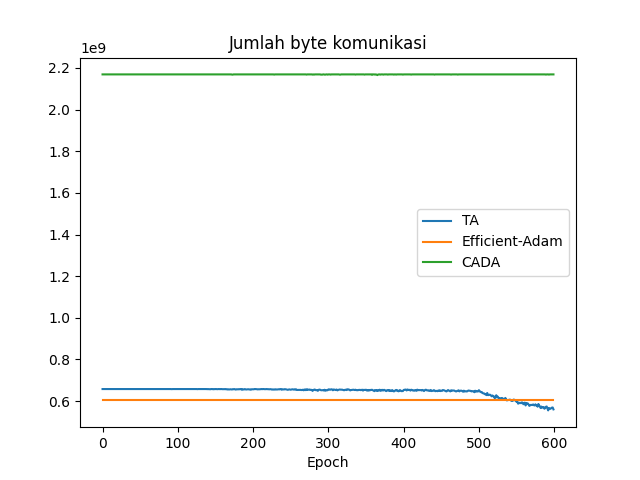
\includegraphics[width=0.8\textwidth]{bits.png}
  \caption{Jumlah byte tiap teknik}\label{bits}
\end{figure}


\subsection{Analisis Hasil Pengujian}
Berdasarkan pengujian yang dilakukan, didapatkan bahwa teknik gabungan dapat menggunakan jumlah byte lebih sedikit dibandingkan CADA, namun lebih banyak dibandingkan Efficient-Adam. Namun, teknik gabungan tetap membutuhkan sedikit lebih banyak byte untuk melakukan komunikasi dibandingkan Efficient-Adam. Penyebab meningkatnya jumlah byte adalah adanya nilai tambahan yang perlu dikomunikasikan oleh \emph{parameter server}, yakni nilai ambang yang digunakan dalam persamaan~\ref{cada2cond}.

Kemudian, jumlah komunikasi yang dilakukan oleh CADA juga masih tidak berkurang sebanyak jumlah komunikasi dalam teknik gabungan. Hal ini mungkin disebabkan karena \emph{hyperparameter} yang dipilih menyebabkan nilai selisih gradien yang didapatkan selalu besar. Dampaknya, persamaan~\ref{cada2cond} tidak pernah terpenuhi. Namun, pemilihan \emph{hyperparameter} lain, seperti menggunakan $\alpha = 0.0005$ menyebabkan model yang dihasilkan memiliki akurasi lebih rendah.

Hasil gabungan yang didapatkan memiliki akurasi yang memiliki akurasi mirip dengan kedua teknik lain. Selain itu, teknik gabungan juga mampu mengurangi kebutuhan komunikasi sejumlah 13.838 ronde dibandingkan Efficient-Adam. Kemudian, hasil gabungan juga dapat mengurangi jumlah byte yang digunakan dalam komunikasi hingga menjadi sekitar 0.303 kali dari CADA.
